\subsection*{Проект СМО}
\addcontentsline{toc}{subsection}{Проект СМО}

\textbf{Задание:}\\
Придумать проект СМО и реализовать его в среде AnyLogic.\\

\textbf{Решение:}\\
Пусть имеется автомойка, которая работает ежедневно. У автомойки есть несколько 10 боксов: 5 боксов осуществляют помывку автомобилей, а другие 5 боксов осуществляют незначительный ремонт автомобилей (замена шин, ремонт фар, $\dots$). Заявки -- автомобили, которые поступают в соответствии с расписанием. Если все боксы заняты, то автомобиль может подождать некоторое время, а может сразу выйти. После обслуживания автомобиль покидает систему.\\

Автомобили могут выйти по времени ожидания в очереди или по количеству заявок, которые накопились в очереди.

В соответствии с описанием выше была построена модель в среде AnyLogic. (Рисунок \ref{fig:car_wash1})
\begin{figure}[h]
	\centering 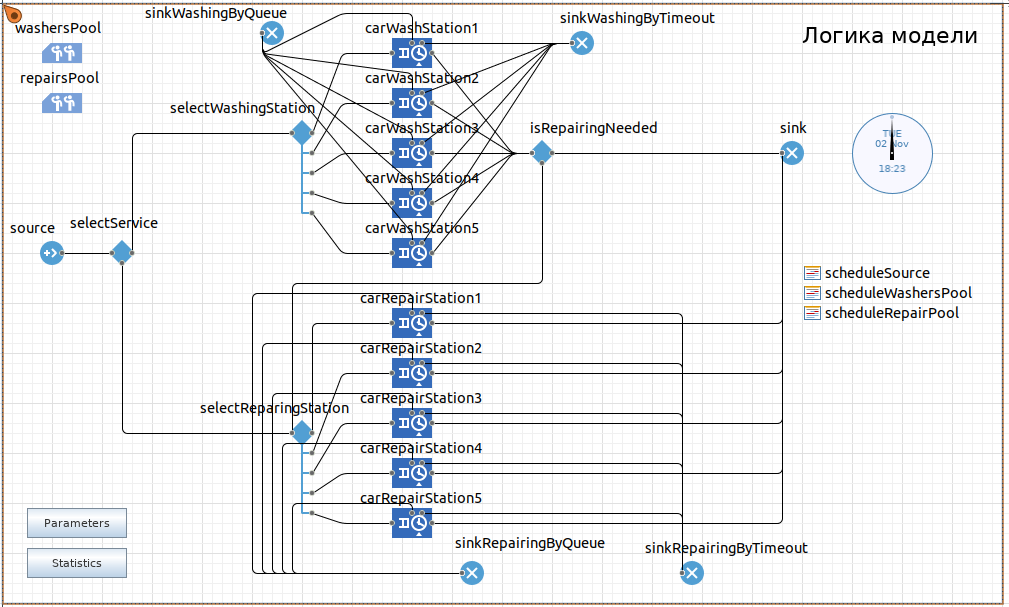
\includegraphics[scale=0.5]{car_wash1}
	\caption{Схема СМО станции технического обслуживания машин}
	\label{fig:car_wash1}
\end{figure}

\newpage

В \textit{Source} заявки поступают в соответствии с расписанием, далее агент с вероятностью 65\% направляется на помывку машины, а может направиться на починку машины. Если агент направился на помывку, то он выбирает наименее загруженный бокс из всех и ждёт своей очереди обслуживания.\\

Предельное время ожидания клиента на помывку машины составляет 120 минут, а предельное количество агентов в очереди для данной услуги составляет 10 человек. Время обслуживания одного клиента было взято с помощью треугольного распределения с параметрами: минимальное время -- 20 минут, мода -- 30 минут, максимальное время -- 50 минут.\\

После того как клиент помыл свою машину, то с вероятностью 25\% он направляется на починку машины. Это стандартная практика для станций технического обслуживания, что перед починкой стоит помыть машину. Если агент направился на починку машины, то он выбирает наименее загруженный бокс из всех и ждёт своей очереди обслуживания.\\

Предельное время ожидания клиента на починку машины составляет 240 минут, а предельное количество агентов в очереди для данной услуги составляет 10 человек. Время обслуживания одного клиента было взято с помощью треугольного распределения с параметрами: минимальное время -- 30 минут, мода -- 40 минут, максимальное время -- 120 минут.\\

Если агент полностью обслужен, то он покидает систему через \textit{Sink}.\\

Из-за того, что на практике агенты поступают с некоторой периодичностью, то было задано расписание для агентов и расписание для сотрудников, которые осуществляют мойку и починку машин. (Рисунок \ref{fig:car_wash2})
\begin{figure}[h]
	\centering 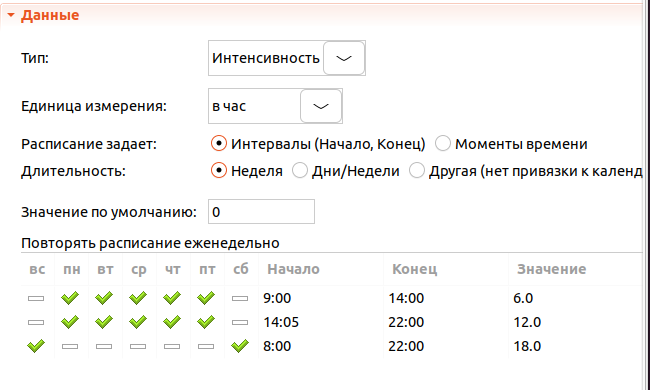
\includegraphics[scale=0.4]{car_wash2}
	\caption{Расписание поступление агентов в систему}
	\label{fig:car_wash2}
\end{figure}

Можно видеть, что в будние дни количество заявок меньше, а в выходные -- больше, что соответствует реальности. В качестве ресурсов в данной модели выступают сотрудники, которые осуществляют мойку и починку автомобилей. Они тоже задавались в соответствии с расписанием.\\

Также в данной модели собиралась статистика о упущенных и обслуженных клиентах по каждому виду сервисов, статистика о загруженности сотрудников по каждому из сервисов. (Рисунок \ref{fig:car_wash3})
\begin{figure}[h]
	\centering 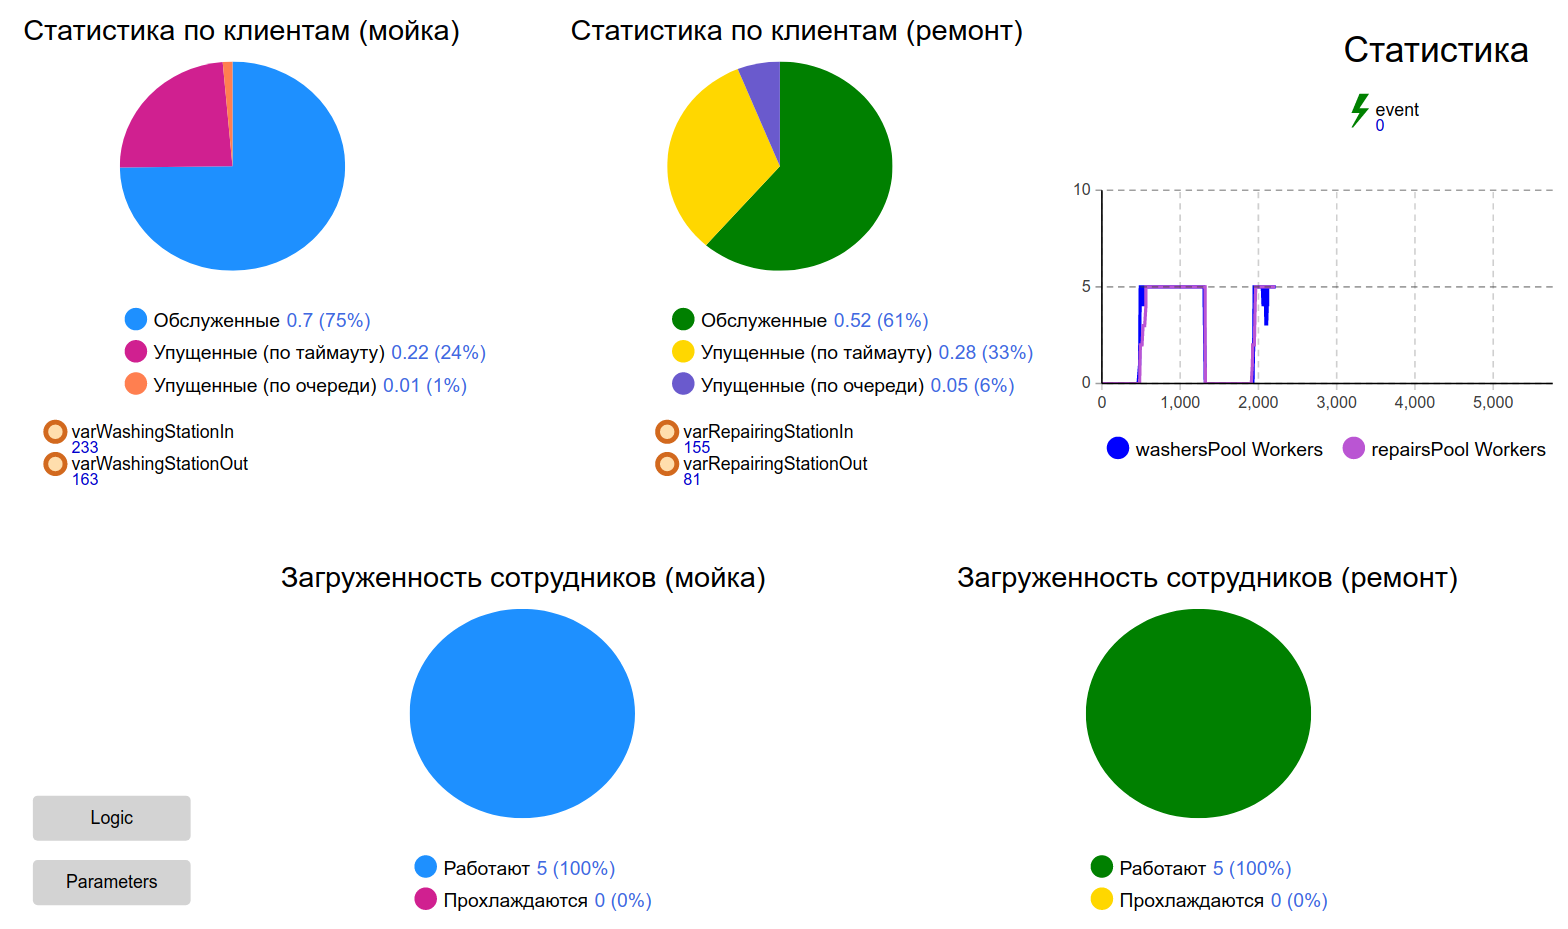
\includegraphics[scale=0.3]{car_wash3}
	\caption{Статистика по модели}
	\label{fig:car_wash3}
\end{figure}

Можно видеть, что при данных параметрах большинство клиентов, примерно 70\%, обслуживаются, а работники полностью загружены. Для уменьшения числа упущенных клиентов стоит сделать больше боксов и соотвественно нанять больше сотрудников для каждого из сервисов.\\

Ещё одним фактором влияющим на число упущенных клиентов является предельное время ожидания клиентов, если его увеличить, то соответственно должно уменьшиться число упущенных клиентов. Аналогичные действия можно предпринять и для увеличения величины очереди.\\

Таким образом, в данной работе удалось промоделировать работу станции технического обслуживания и проанализировать показатели модели.\\